\documentclass[conference]{IEEEtran}
%+++++++++++++++++++++++++++++++++++++++++++
% Added to commands
\input epsf
\usepackage{graphicx}
\usepackage [french]{babel}
\usepackage [utf8]{inputenc}
\usepackage [T1] {fontenc}
\usepackage{float}
%+++++++++++++++++++++++++++++++++++++++++++
% correct bad hyphenation here
\hyphenation{op-tical net-works semi-conduc-tor IEEEtran}
\begin{document}

%+++++++++++++++++++++++++++++++++++++++++++
\title{\LARGE Etude de l'influence du couple (diamètre, profondeur) sur la finesse d'un kite
\vskip10pt

\small 2024 - Romain LAMBERT
}
%+++++++++++++++++++++++++++++++++++++++++++
% make the title area
\maketitle

\begin{abstract}Ce bureau d'étude a pour sujet l'étude de l'influence du \textbf{diamètre} (diameter) et de la \textbf{cambrure} (depth) sur la finesse d'un kite. L'objectif final étant de déterminer un couple (t,k) = (diameter, depth) qui serve de référence pour le dimensionnement des kites. Aussi, cette étude permet d'évaluer la sensibilité de la \textbf{VSM} sous la théorie 2D de la \textbf{regression de Breukels} à ces deux paramètres.
\end{abstract}
\IEEEoverridecommandlockouts

\IEEEpeerreviewmaketitle
\section{La théorie}

\subsection{\textbf{Regresion de Breukels : théorie 2D}} 

Si la VSM permet d'étudier l'aérodynamique 3D d'un kite, elle requiert le calcul des coefficients 2D de chaque section($C_L$, $C_D$, $C_M$). Afin de limiter le coût de calcul et de se baser sur des polaires adaptées à des profils "non conventionnels", la VSM utilise une \underline{formule de regression de Breukels}. 
Cette formule est issue de résultats obtenus sur des profils typiques de kites à boudin, et ne \underline{dépend que du diamètre du boudin et de la cambrure du profil}. \\


\begin{center}
    \begin{equation}
        C_L = \lambda_5  \alpha^3 +\lambda_6  \alpha^2 + \lambda_7  \alpha + \lambda_8
        \label{eq:Cl_breukels}
    \end{equation}
\end{center}
avec :
\begin{center}
    \begin{equation}
        \lambda_i = S_x  k + S_y
        \label{eq:lamba_breukels}
    \end{equation}
\end{center}
et :
\begin{center}
    \begin{equation}
        S_i = C_x  t^2 + C_y  t + C_z
        \label{eq:S_breukels}
    \end{equation}
\end{center}
où les 23 coéfficients $C_x$ sont prédéterminés, et (t,k) est le couple (diamètre, cambrure) définit tel que :
\begin{center}
    \begin{equation}
        t = \frac{Diamètre(BA)}{Corde} ; k = \frac{max(CoordonéesExtrados)}{Corde}
        \label{eq:tk_breukels}
    \end{equation}
\end{center}

Ainsi, l'obtention ds coéfficients 2D permet ensuite à la VSM d'ajouter l'indluence des effets 3D (loi de corde, d'envergure, de voute...) sur les coefficients aérodynamiques d'un kite

\begin{figure}[H]
    \centering
    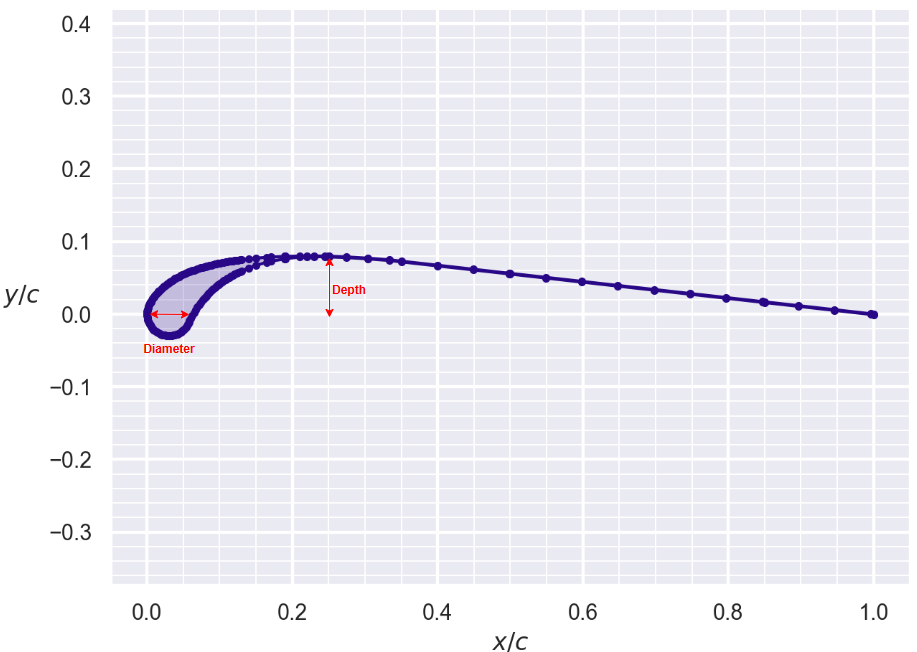
\includegraphics[width=0.5\textwidth]{Pics/airfoil.png}  
    \caption{Profil central d'une SK50-VG avec identification du diamètre et de la cambrure tel que utilisés par la VSM.}
    \label{fig:airfoil}
\end{figure}

%%%%%%%%%%%%%%%%%%%%%%%%%%%%%%%%%%%%%%%%%%%%%%%%%%%%%%%%%%%%%%%%%%%%%%%%%
\IEEEpeerreviewmaketitle
\section{Le Code }

\subsection{Le cas d'étude - 2D} 

On étudie dans un premier temps La fonction de Breukels pour en chercher les optimum. On utilise pour ce faire un code d'optimsiation fournit par la bibliothèque \textbf{aerosandbox} et on se place dans deux cas d'optimisation : 
\begin{itemize}
    \item Maximum de $\frac{C_L(\alpha)}{C_D(\alpha)}$ à angle $\alpha$ fixé 
    \item Maximum de $\sum_{\alpha = 0}^{20}\frac{C_L(\alpha)}{C_D(\alpha)} Gaussienne(alpha, center, sigma) $
\end{itemize}

    où $Gaussienne(\alpha, center, \sigma) = e^{-\frac{(center - \alpha)^2}{2\sigma^2}}$ est une Gaussienne permettant d'obtenir une moyenne pondérée. 

\textbf{Pour notre étude, on choisit Center = 7° et sigma = 8}. Les résultats sont présentés dans la partie suivante.
\begin{figure}[H]
    \centering
    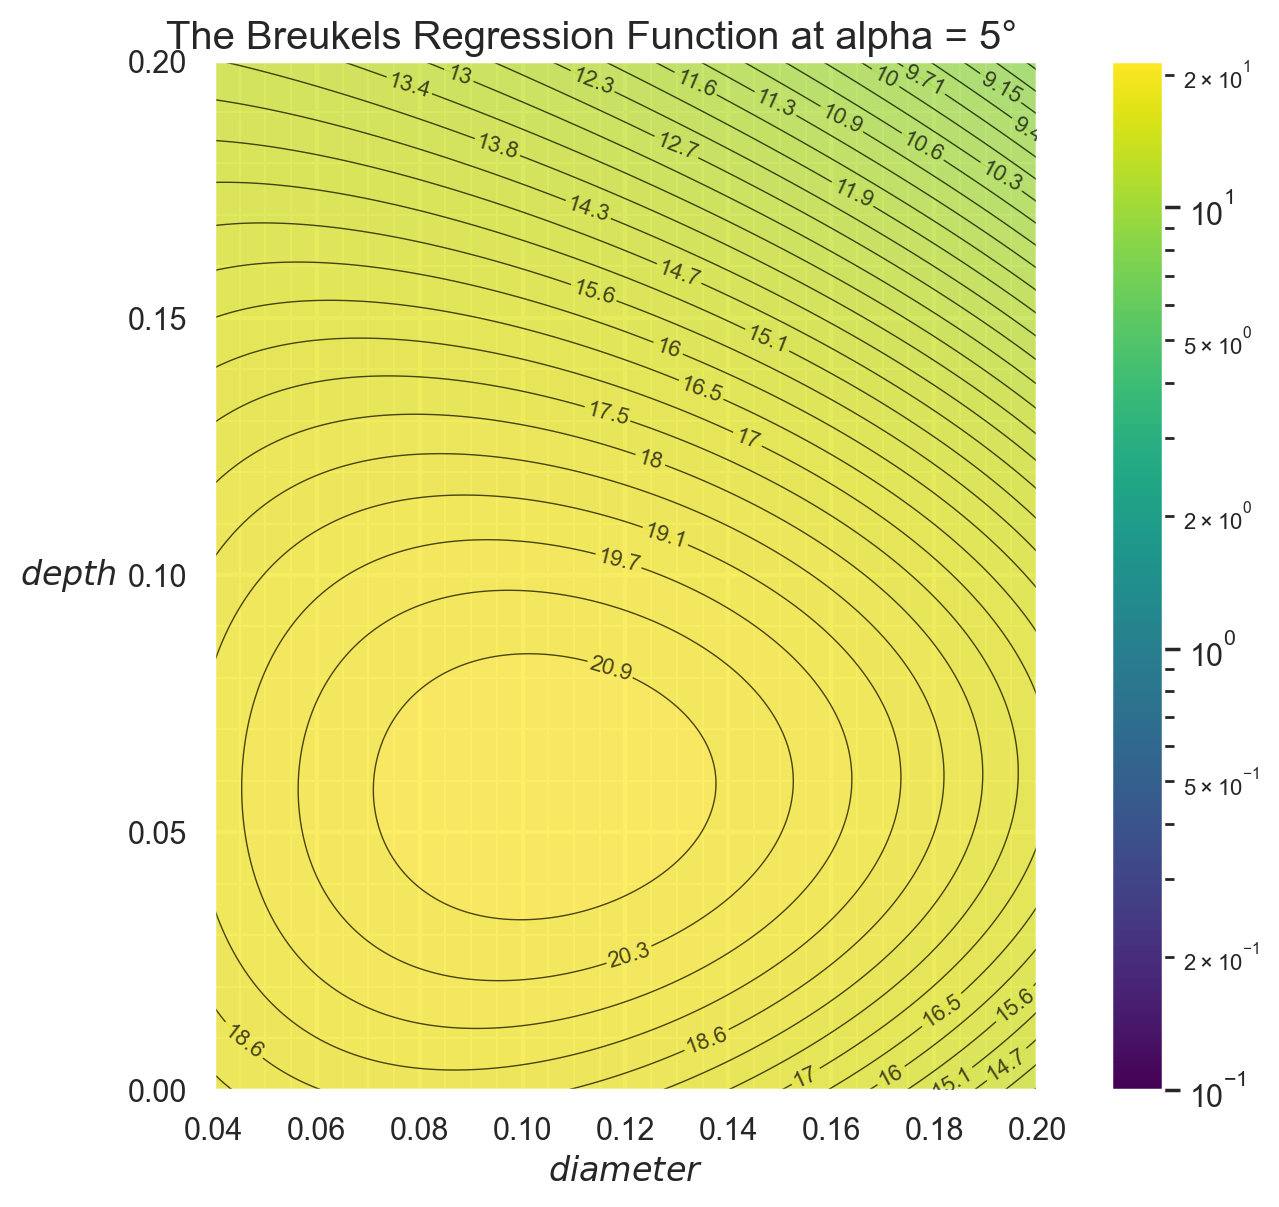
\includegraphics[width=0.5\textwidth]{Pics/breukels.png}  
    \caption{Tracer de $\frac{C_L}{C_D}$ par Régression de Breukels à $\alpha$=5°}
    \label{fig:breukels}
\end{figure}


\subsection{Le cas d'étude - 3D} 

On se place ensuite dans le cas d'étude d'un SK50-VG dont on fait varier le \textbf{diamètre t entre -0.02 et +0.1 et la cambrure k entre -0.1 et 0.1}. \\
    A noter que sur chaque section de l'aile \textbf{le diamètre ne peut pas être inférieur à 0.04 et la cambrure inférieur au demi-diamètre}. Ainsi, les résultats sont à nuancer : \textbf{une aile avec un certain delta de t ou de k ne veut as dire que toutes les sections ont été modifiées de ce delta; seules les sections respectant ces critères de minimum énoncés précédemment le sont.}

La loi d'évolution de t et k sur une VG est initialement:  
\begin{itemize}
    \item t : [0.07 0.067 0.065 0.063 0.061 0.06 0.06  0.06 0.06 0.06  0.06  0.06 0.06 0.06  0.06 0.061 0.063 0.065 0.067 0.07]
    \item k : [0.034 0.05 0.0645 0.0686 0.072 0.075 0.08 0.08 0.08 0.08      0.08 0.08 0.08 0.08 0.075 0.072 0.0686 0.0645 0.05 0.034]
\end{itemize}

    A nouveau, on cherche l'optimum dans les 2 problèmes d'optimisation suivants:
    \begin{itemize}
        \item Maximum de $\frac{C_L(\alpha)}{C_D(\alpha)}$ à angle $\alpha$ fixé 
        \item Maximum de $\sum_{\alpha = 0}^{21}\frac{C_L(\alpha)}{C_D(\alpha)} Gaussienne(alpha, center, sigma) $
    \end{itemize}
    Les résultats sont présentés dans la partie suivante.

\begin{figure}[H]
    \centering
    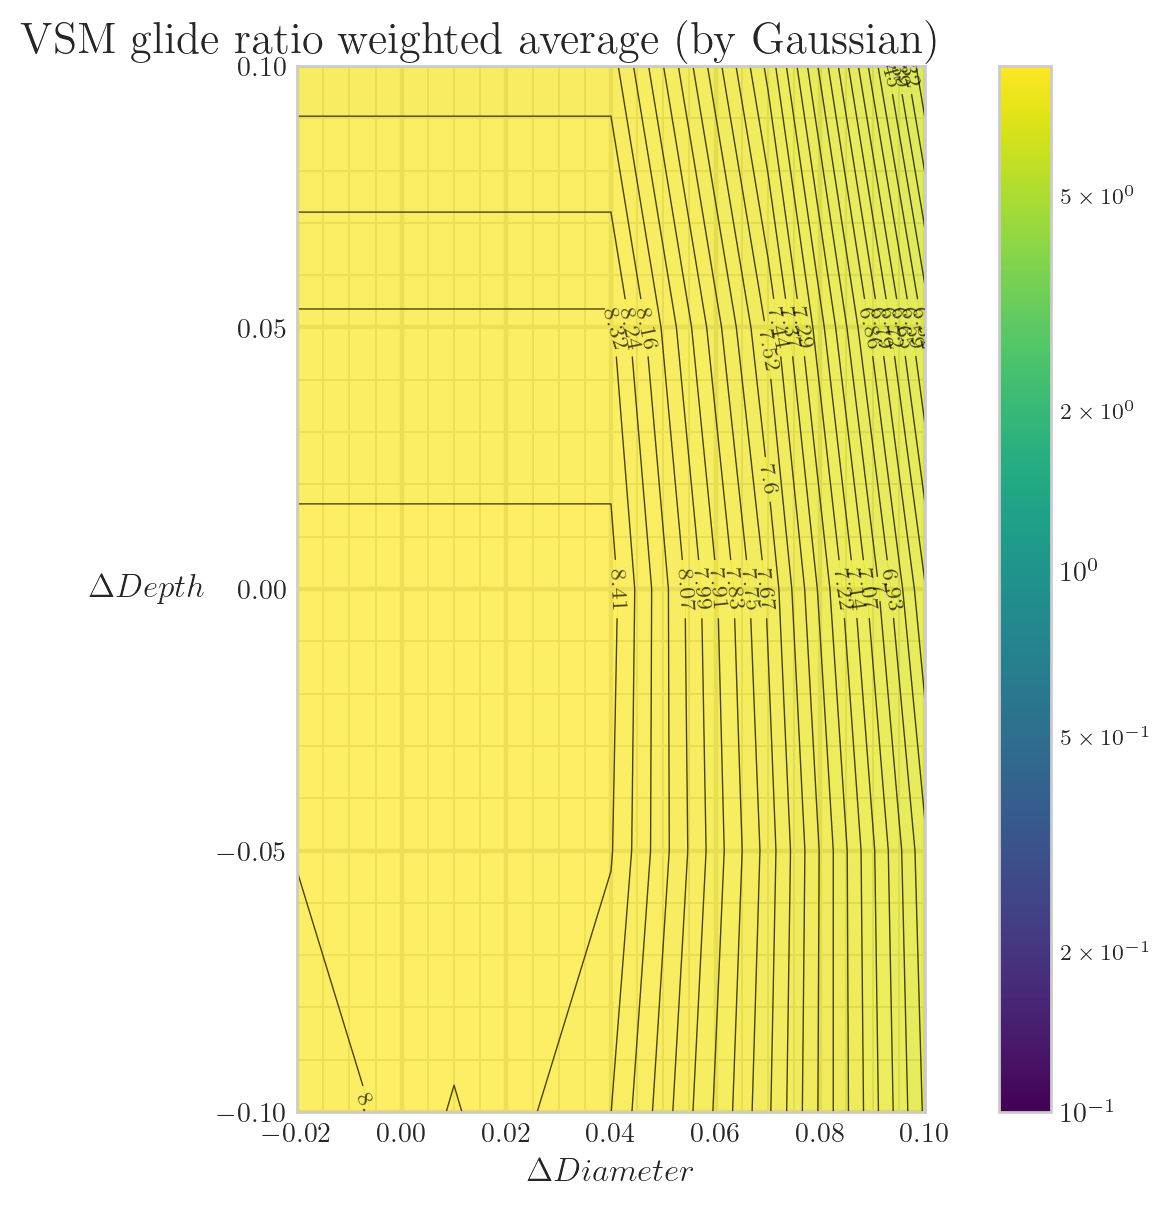
\includegraphics[width=0.5\textwidth]{Pics/vsm.png}  
    \caption{Tracer de $\frac{C_L}{C_D}$ par VSM en faisant varier (t,k)}
    \label{fig:vsm}
\end{figure}


%%%%%%%%%%%%%%%%%%%%%%%%%%%%%%%%%%%%%%%%%%%%%%%%%%%%%%%%%%%%%%%%%%%%%%%%%
\IEEEpeerreviewmaketitle
\section{Les Résultats}

\subsection{2D - résultats par $\alpha$}

\[
\begin{array}{|c|c|c|}
    \hline
    \textbf{$\alpha$} & \textbf{diamètre} & \textbf{cambrure}\\
    \hline
    0 & 0.040 & 0.20 \\
    1 & 0.091 & 0.00 \\
    2 & 0.098 & 0.00 \\
    3 & 0.10 & 0.01  \\
    4 & 0.10 & 0.04  \\
    5 & 0.10 & 0.06  \\
    6 & 0.10 & 0.068  \\
    7 & 0.095 & 0.074 \\
    8 & 0.089 & 0.078 \\
    9 & 0.079 & 0.082 \\
    10 & 0.061 & 0.086 \\
    11 & 0.040 & 0.093 \\
    12 & 0.040 & 0.103 \\
    13 & 0.040 & 0.105 \\
    14 & 0.040 & 0.107 \\
    15 & 0.040 & 0.109 \\
    16 & 0.040 & 0.111 \\
    17 & 0.040 & 0.113 \\
    18 & 0.040 & 0.115 \\
    19 & 0.040 & 0.118 \\
    20 & 0.040 & 0.121 \\
    \hline
\end{array}
\]

\begin{figure}[H]
    \centering
    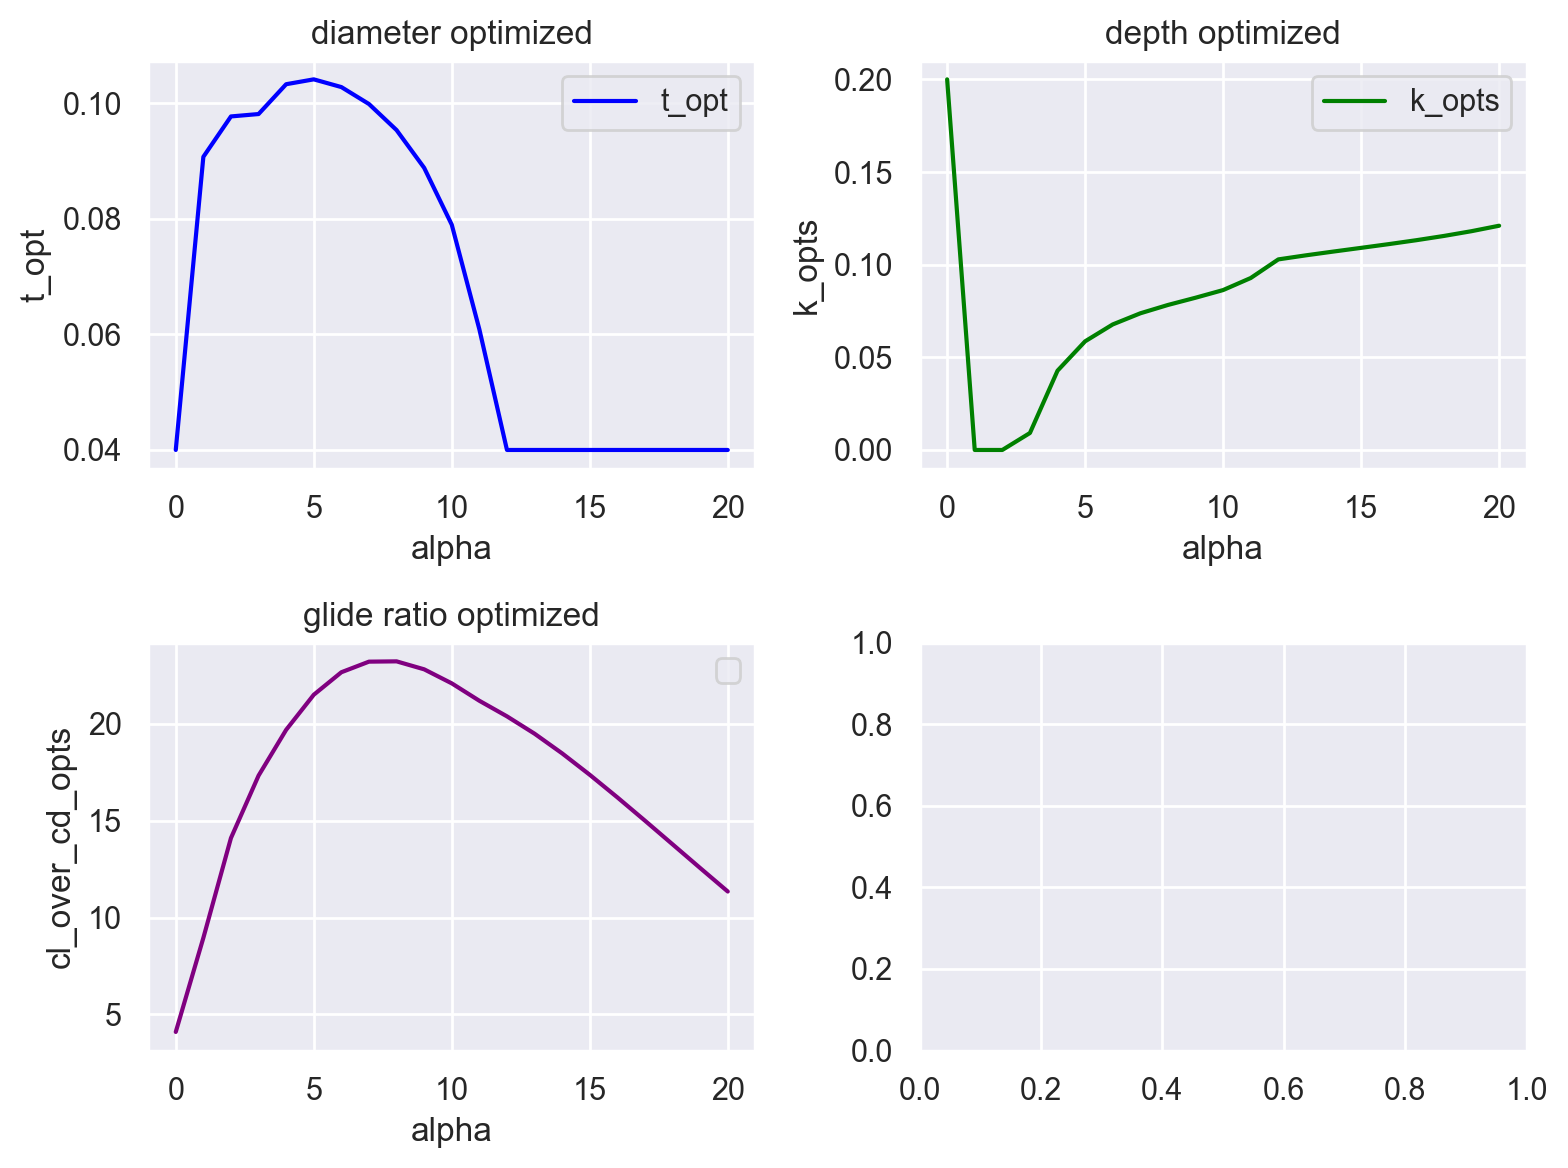
\includegraphics[width=0.5\textwidth]{Pics/résultats pas alpha 2D.png}  
    \caption{Tracer de t et k optimaux pour chaque alpha}
    \label{fig:t,k,alpha 2d}
\end{figure}

    \textbf{Remarque :} 
    \begin{itemize}
        \item On observe que pour les grands angles le diamètre optimal tend à être le plus petit possible.
        \item La cambrure optimale augmente avec $\alpha$.
        \item Les résultats sont cohérents en ordre de grandeur
    \end{itemize}

\subsection{2D - résultats avec moyenne pondérée par Gaussienne}

    Avec une Gaussienne de paramètres \textbf{center = 7° et sigma = 8}, les valeurs qui maximisent la fonction objective (moyenne pondérée de finesse aérodynamique) sont :
    \begin{itemize}
        \item t : 0.0745
        \item k : 0.0860
    \end{itemize}
    \textbf{Ces résultats sont cohérents en ordre de grandeur.}

\subsection{3D - résultats par $\alpha$}

Le tableau suivant présente les résultats obtenu avec la VSM (3D). Les nombres de ribs saturés en diamètre/cambrure sont, pour chaque alpha, les nombre de ribs qui ne pouvaient pas atteindre la valeurs objective (Valeurs initiale + delta) et qui donc sont "saturés" à la valeurs minimal ( $\frac{Diamètre}{2}$ pour la cambrure et 0.04 pour le diamètre).\\

A noter que les ribs initialement à faible diamètre (relatif) sont ceux du bord d'attaque, et que les profils les moins cambré sont aux tips; en témoigne les valeurs initiales de t et k présentés en II.B..

\[
\begin{array}{|c|c|c|c|c|}
    \hline
    \textbf{$\alpha$} & \textbf{$\delta diametre$} & \textbf{nombre ribs saturés en diamètre} & \textbf{$\delta cambrure$} & \textbf{nombre ribs saturés en cambrure}\\
    \hline
    0 & -0.02 & 10 & -0.1 & 20\\
    1 & -0.007 & 0 & -0.1 & 20\\
    2 & -0.007 & 0 & -0.1 & 20\\
    3 & -0.007 & 0 & -0.1 & 20 \\
    4 & -0.007 & 0 & -0.1 & 20 \\
    5 & -0.007 & 0 & -0.1 & 20 \\
    6 & -0.007 & 0 & -0.1 & 20  \\
    7 & -0.007 & 0 & -0.1 & 20 \\
    8 & -0.02 & 0 & -0.1 & 20 \\
    9 & -0.02 & 0 & -0.1 & 20 \\
    10 & -0.02 & 0 & -0.1 & 20 \\
    11 & 0.033 & 0 & -0.033 & 12 \\
    12 & 0.033 & 0 & -0.033 & 12 \\
    13 & 0.033 & 0 & -0.1 & 4 \\
    14 & 0.02 & 0 & -0.1 & 4 \\
    15 & 0.02 & 0 & -0.1 & 4 \\
    16 & 0.02 & 0 & -0.1 & 4 \\
    17 & 0.02 & 0 & -0.1 & 4 \\
    18 & -0.007 & 0 & 0.1 & 0 \\
    19 & -0.007 & 0 & 0.1 & 0 \\
    20 & -0.007 & 0 & 0.1 & 0 \\
    \hline
\end{array}
\]
    \textbf{Remarque :}
    \begin{itemize}
        \item Pour beaucoup de valeurs optimales, un nombre importants de ribs sont saturés en cambrure
        \item Le faible nombre d'échantillon semble limité la précision des résultats. Avec 10 valeurs de $\delta Diameter$ et 10 valeurs de $\delta Depth$, on est déjà à 10x10 = 100 simulations (45 minutes)!
    \end{itemize}

\subsection{3D - résultats avec moyenne pondérée par Gaussienne}
Avec une Gaussienne de paramètres \textbf{center = 7° et sigma = 8}, les valeurs qui maximisent la fonction objective (moyenne pondérée de finesse aérodynamique) sont :
\begin{itemize}
    \item $\delta diameter$ : 0.02
    \item $\delta depth$ : -0.1
\end{itemize}

\textbf{Les valeurs de diamètre et cambrure optimaux ainsi obtenus en 3D sont : 
}

\begin{itemize}
    \item t : 0.090 0.086 0.085 0.083 0.081 0.080 0.080  0.080 0.080 0.080 0.080  0.080 0.080 0.080 0.080 0.081 0.083 0.085 0.087 0.090
    \item k : 0.045 0.043 0.043 0.041 0.040 0.040 0.040  0.040 0.040 0.040 0.040 0.040 0.040 0.040  0.040 0.040 0.041 0.043 0.043 0.045
\end{itemize}

\textbf{A comparer avec les valeurs initiales :}
\begin{itemize}
    \item t : 0.07 0.067 0.065 0.063 0.061 0.06 0.06  0.06 0.06 0.06  0.06  0.06 0.06 0.06  0.06 0.061 0.063 0.065 0.067 0.07
    \item k : 0.034 0.05 0.0645 0.0686 0.072 0.075 0.08 0.08 0.08 0.08 0.08 0.08 0.08 0.08 0.075 0.072 0.0686 0.0645 0.05 0.034
\end{itemize}

\textbf{On note donc une tendance (en 3D) à augumenter diamètre et cambrure du kite. }\\
A noter que l'étude est réalisée à \textbf{50 knots}. 

\section{ Limites et Etudes Complémentaires}

Tout d'abord Breukels ne prend en compte que le diamètre et la cambrure maximal d'un profil, \textbf{la position de la cambrure maximale d'un profil n'est donc pas prise en compte}. \\

Ensuite, l'étude réalisée \textbf{ne fait pas intervenir de critère de stabilité.} Il sera sujet par suite d'une telle étude avec les résultats obtenus dans ce papier.\\

De plus, le choix de la fonction objective pour la recherche d'un optimum (moyenne pondérée par une Gaussienne) est peu justifiée. Connaître la valeurs d'un angle d'attaque pour lequel on souhaite optimiser une fonction ( finesse, stabilité, portance...) permettrait d'avoir un résultat plus pertinant. \textbf{Mesurer les angles d'attaques principaux lors des essais kite, peut-être avec l'extended Karmann Filter (EKF)} fournit par Kite Power, permettrait de répondre à ce problème. Le choix de sigma et alpha center dans la Gaussienne sont, eux aussi, criticables.\\

Finalement les fonctions d'optimisation d'Aerosandbox ne sont pas applicables à la VSM. Elles sont cependant utilisées pour optimiser la fonction de Breukels (2 paramètres) et les profils représentés avec 10 paramètres (Kulfan parameters) tel quel :  

\begin{figure}[H]
    \centering
    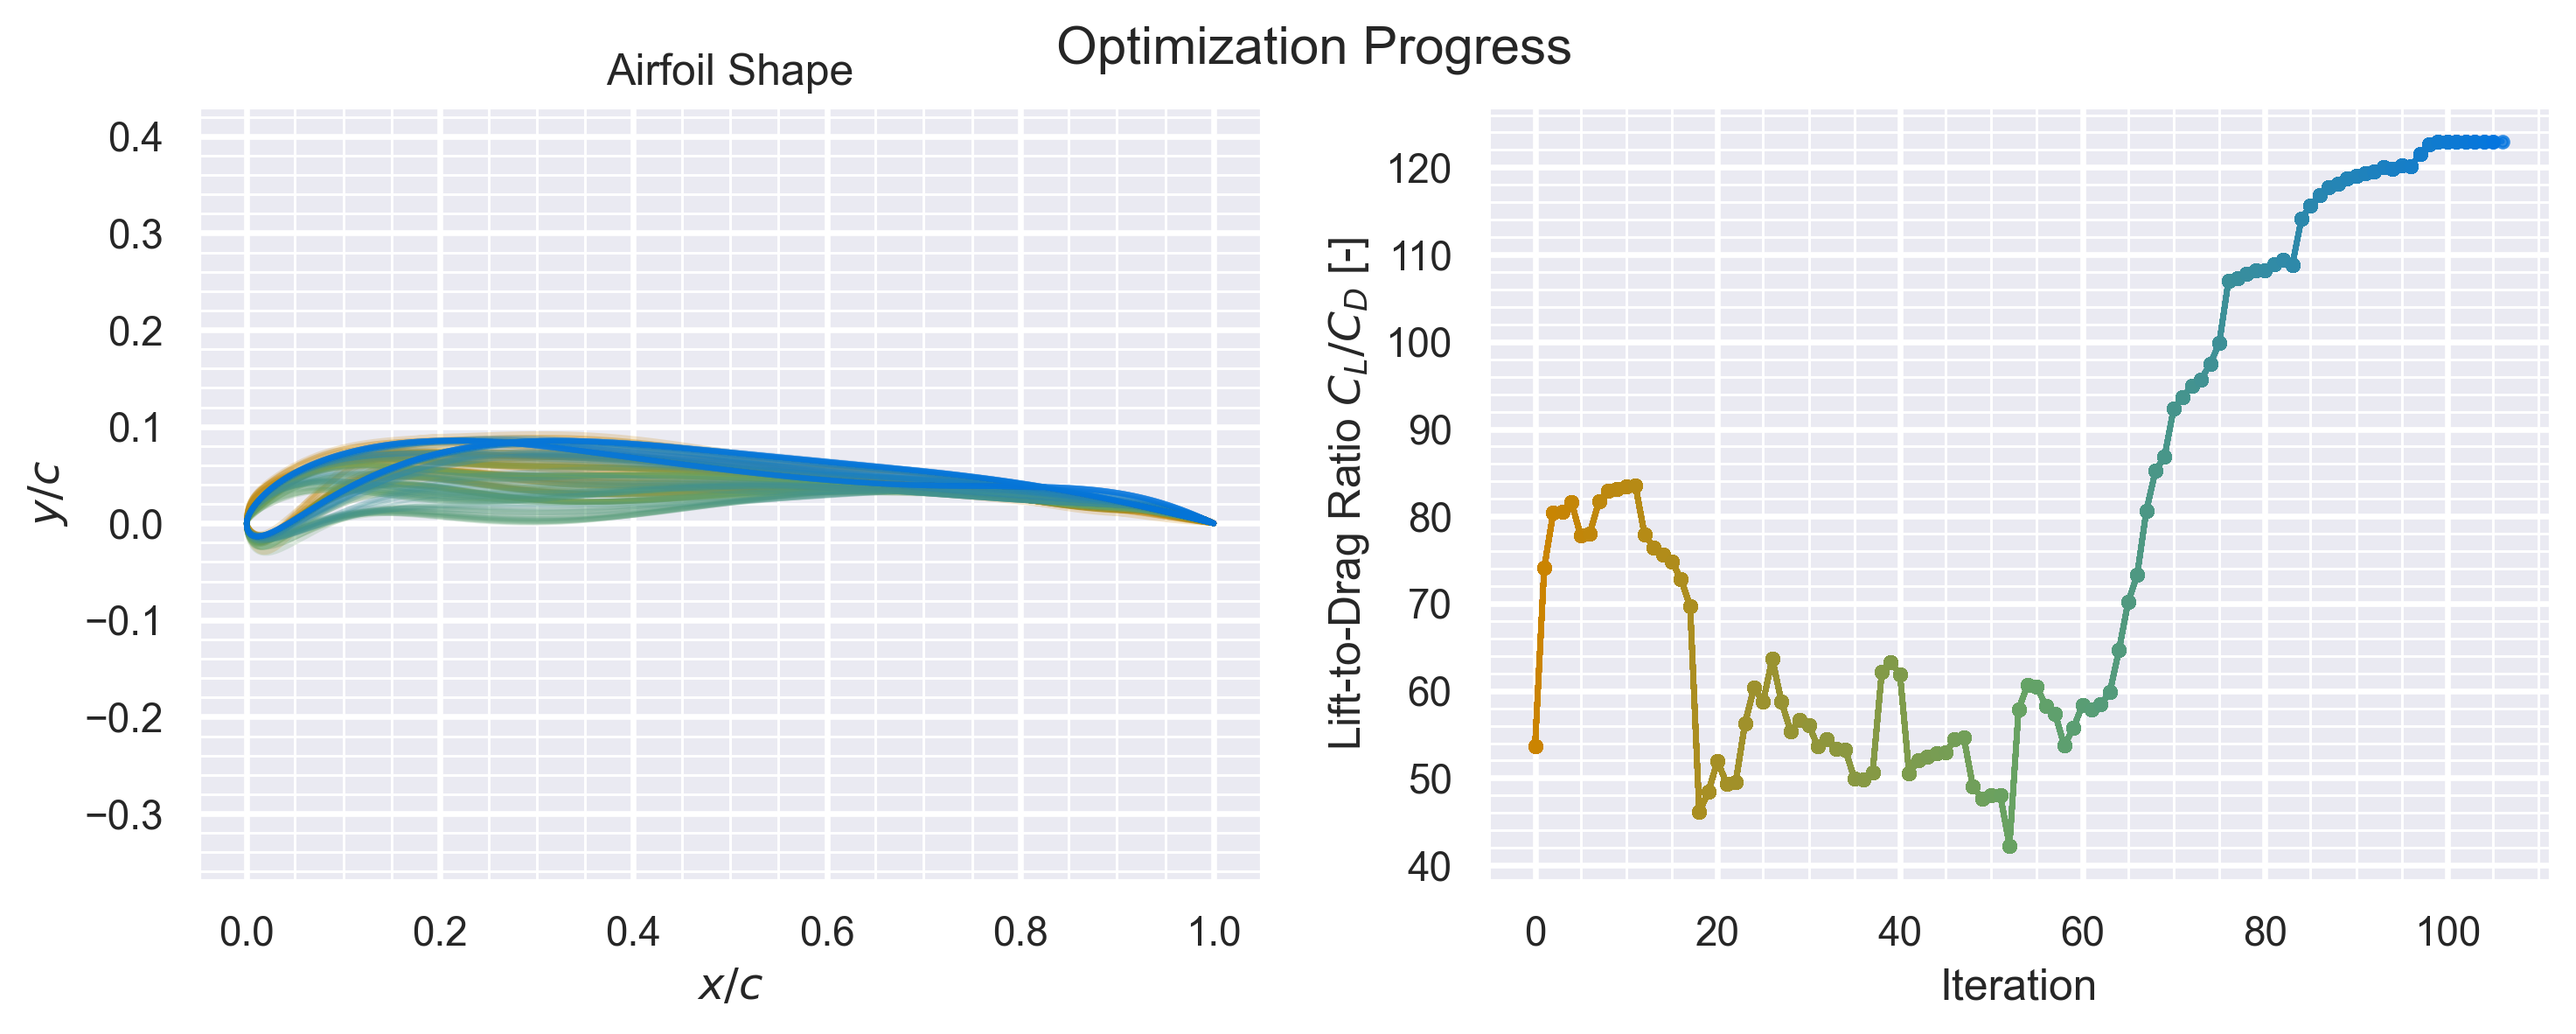
\includegraphics[width=0.5\textwidth]{Pics/optim neuralfoil.png}  
    \caption{Optimisation réalisée avec Aerosandbox sur des profils dis "de Kulfan"}
    \label{fig:kulfan}
\end{figure}


\end{document}